\documentclass[a4paper]{article}
\usepackage[pdftex]{hyperref}
\usepackage[latin1]{inputenc}
\usepackage[english]{babel}
\usepackage{a4wide}
\usepackage{amsmath}
\usepackage{amssymb}
\usepackage{algorithmic}
\usepackage{algorithm}
\usepackage{ifthen}
\usepackage{listings}
\usepackage{array}
\usepackage{tabu}
% move the asterisk at the right position
\lstset{basicstyle=\ttfamily,tabsize=4,literate={*}{${}^*{}$}1}
%\lstset{language=C,basicstyle=\ttfamily}
\usepackage{moreverb}
\usepackage{palatino}
\usepackage{multicol}
\usepackage{tabularx}
\usepackage{comment}
\usepackage{verbatim}
\usepackage{color}
\usepackage{graphicx}
\usepackage{array,mathtools}
\usepackage{amsmath}

%% pdflatex?
\newif\ifpdf
\ifx\pdfoutput\undefined
\pdffalse % we are not running PDFLaTeX
\else
\pdfoutput=1 % we are running PDFLaTeX
\pdftrue
\fi
\ifpdf
\fi
\ifpdf
\DeclareGraphicsExtensions{.pdf, .jpg}
\else
\DeclareGraphicsExtensions{.eps, .jpg}
\fi

\parindent=0cm
\parskip=0cm

\setlength{\columnseprule}{0.4pt}
\addtolength{\columnsep}{2pt}

\addtolength{\textheight}{5.5cm}
\addtolength{\topmargin}{-26mm}
\pagestyle{empty}

%%
%% Sheet setup
%% 
\newcommand{\coursename}{Computer Architecture and Programming Languages}
\newcommand{\courseno}{CO20-320241}
\newcommand*{\carry}[1][1]{\overset{#1}}
\newcolumntype{B}[1]{r*{#1}{@{\,}r}}
 
\newcommand{\sheettitle}{Homework}
\newcommand{\mytitle}{}
\newcommand{\mytoday}{{21st of October}, 2019}

% Current Assignment number
\newcounter{assignmentno}
\setcounter{assignmentno}{6}

% Current Problem number, should always start at 1
\newcounter{problemno}
\setcounter{problemno}{1}

%%
%% problem and bonus environment
%%
\newcounter{probcalc}
\newcommand{\problem}[2]{
  \pagebreak[2]
  \setcounter{probcalc}{#2}
  ~\\
  {\large \textbf{Problem \textcolor{blue}{\arabic{assignmentno}}.\textcolor{blue}{\arabic{problemno}}} \hspace{0.2cm}\textit{#1}} \refstepcounter{problemno}\vspace{2pt}\\}

\newcommand{\bonus}[2]{
  \pagebreak[2]
  \setcounter{probcalc}{#2}
  ~\\
  {\large \textbf{Bonus Problem \textcolor{blue}{\arabic{assignmentno}}.\textcolor{blue}{\arabic{problemno}}} \hspace{0.2cm}\textit{#1}} \refstepcounter{problemno}\vspace{2pt}\\}

%% some counters  
\newcommand{\assignment}{\arabic{assignmentno}}

%% solution  
\newcommand{\solution}{\pagebreak[2]{\bf Solution:}\\}

%% Hyperref Setup
\hypersetup{pdftitle={Homework \assignment},
  pdfsubject={\coursename},
  pdfauthor={},
  pdfcreator={},
  pdfkeywords={Computer Architecture and Programming Languages},
  %  pdfpagemode={FullScreen},
  %colorlinks=true,
  %bookmarks=true,
  %hyperindex=true,
  bookmarksopen=false,
  bookmarksnumbered=true,
  breaklinks=true,
  %urlcolor=darkblue
  urlbordercolor={0 0 0.7}
}

\begin{document}


\coursename \hfill Course: \courseno\\
Jacobs University Bremen \hfill \mytoday\\
Fjolla Dedaj\hfill
\vspace*{0.3cm}\\
\begin{center}
{\Large \sheettitle{} \textcolor{blue}{\assignment}\\}
\end{center}
\problem{}{0}
\\
\textbf{In the register instruction format (used e.g., for add), the fields rs, rt, and rd occupy 5 bits each. Why are they 5 bits wide, and not 4 or 6 or some other value?}\\
\\
\solution
Because in total, we have 32 registers (0 - 31) and 5 bits are enough to represent them in binary ($31_{10} = 11111_{2}$) using the GNU MIPS register allocation.\\
\problem{}{0}
\solution\\
\textbf{a)} op ($operation$) = 0, rs ($source 1$)= 8, rt ($source 2$) = 9, rd ($destination$) = 10, shamt ($shift$) = 0, funct ($operation$) = 34\\
\\
Since funct = 34 and op = 0, we have a subtraction instruction. Also, because 8 = \$t0, 9 = \$t1 and 10 = \$t2, the instruction is as follows:
\begin{center}
\textbf{sub \$t2, \$t0, \$t1}\\ 
\end{center}
\textbf{b)} op = 0x23, rs = 17, rt = 18, const = 0x4\\
\\
$23_{26} = 3 * 16^0 + 2 * 16^1 = 3 + 32 = 35_{10}$\\
rs (source 1) = 17 = \$s1\\
rt (source 2) = 18 = \$s2\\
op = $0x23 = 35_{10} =$ lw\\
\\Thus, the instruction is:
\begin{center}
\textbf{lw \$s1, 4(\$s2)}\\
\end{center}
\problem{}{0}
\solution\\
\textbf{a)} op = 0, rs = 8, rt = 9, rd = 10, shamt = 0, funct = 34\\
\\
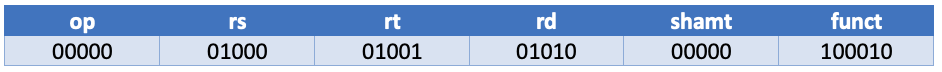
\includegraphics[scale=0.5]{problem3a.png}\\
\\
\textbf{rs} $= 8_{10} = 01000_{2}$\\
\textbf{rt} $= 9_{10} = 01001_{2}$\\
\textbf{rd} $= 10_{10} = 01010_{2}$\\
\textbf{funct} $= 34_{10} = 100010_{2}$\\
\\
\textbf{b)} op = 0x23, rs = 17, rt = 18, const = 0x4\\
\\
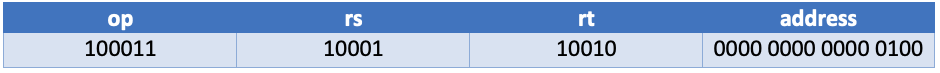
\includegraphics[scale=0.46]{problem3b.png}\\
\\
\textbf{op} = 0x23 $= 35_{10} = 100011_{2}$\\
\textbf{rs} $= 17_{10} = 10001_{2}$\\
\textbf{rt} $= 18_{10} = 10010_{2}$\\
\textbf{const} = 0x4 $= 4_{10} = 0000$ $0000$ $0000$ $0100_{2}$\\
\\
\pagebreak
\\
\problem{}{0}
.\qquad slt \$t2, \$t0, \$t1\\
.\qquad      beq \$t2, \$0, ELSE\\
.\qquad      j DONE\\
ELSE: addi \$t2, \$0, 2\\
DONE:\\
\\
$\textbf{\$t0} = 0010$ $0100$ $1001$ $0010$ $0100$ $1001$ $0010$ $0100_{2} = 613566756_{10}$\\
$\textbf{\$t1} = 0011$ $1111$ $1111$ $1000$ $0000$ $0000$ $0000$ $0000_{2} = 1073217536_{10}$\\
\\
\solution\\
\textbf{slt \$t2, \$t0, \$t1} \qquad if(\textbf{\$t0} $<$ \textbf{\$t1}) \textbf{\$t2} = 1 else \textbf{\$t2} = 0\\
.\qquad \qquad \qquad \qquad \qquad Since \textbf{\$t0} $<$ \textbf{\$t1}, \textbf{\$t2} = 1\\
\\
\textbf{beq \$t2, \$0, ELSE} \qquad if(\textbf{\$t2} $==$ \textbf{\$0}) goto ELSE\\
.\qquad \qquad \qquad \qquad \qquad Since \textbf{\$t2} != 0 we don't go to \textbf{ELSE} but we jump to \textbf{DONE}.\\
.\qquad \qquad \qquad \qquad \qquad Thus, the value of \textbf{\$t2} remains 1.\\
\problem{}{0}
\solution
\textbf{Offset}: A[i] = 4 * i, thus: A[6] = 4 * 6 = 24.\\
\\
lw \$t0, 24(\$s0)\\
add \$t0, \$t0, \$s0\\
lw \$t1, 0(\$t0)\\
add \$t1, \$t1, \$s1\\
sw, \$t1, 0(\$t0)
\\
\problem{}{0}
\solution\\
lui \$s4 35 \qquad (load upper immediate)\\
ori \$s4, \$s4, 35 \qquad (bitwise logical OR)\\
\problem{}{0}
\solution\\
. \qquad \qquad li \$t0, 0 $\Longrightarrow$  load immediate for $i$\\
. \qquad \qquad li \$t1, 8 $\Longrightarrow$  load immediate for the limit of $i$\\
LOOP:\qquad beq \$t0, \$t1, END $\Longrightarrow$ if (\$t0 == \$t1) go to \textbf{END}, else $\rightarrow$  execute the instructions below\\
. \qquad \qquad addi \$s0, \$s0, 4 $\Longrightarrow$ add 4 to a\\
. \qquad \qquad addi \$t0, \$t0, 1 $\Longrightarrow$ add 1 to i\\
. \qquad \qquad j LOOP $\Longrightarrow$ jump to the start of the loop again\\
END: ...
\end{document}